%% Ankur Sinha

%% packages %%
% support for coloured text
\usepackage{color}
% IPA
\usepackage{tipa}
\usepackage[scale=2]{ccicons}
\usepackage{amssymb}
\usepackage{tikz}
\usetikzlibrary{arrows.meta, arrows}
\usepackage{jneurosci}
\usepackage{subfig}
\usepackage[T1]{fontenc}
\usepackage[utf8]{inputenc}
\usepackage[style=verbose,backend=biber,autocite=footnote]{biblatex}
\addbibresource{/home/asinha/Documents/01_Readables/00_research_papers/masterbib.bib}
% Use opensans
\usepackage[default,osfigures,scale=0.95]{opensans}
% for strike through
\usepackage[normalem]{ulem}
% links, urls, refs
\definecolor{links}{HTML}{2A1B81}
% Fedora blue for the theme
\definecolor{FedoraBlue}{HTML}{2A1B81}
\usepackage{hyperref}
\hypersetup{colorlinks,linkcolor=Green,urlcolor=links}
% graphics
\usepackage{graphicx}
% algorithm
\usepackage{algorithmic}
\usepackage{textcomp}
\usepackage{wrapfig}
\usepackage{textgreek}
\usepackage{euler}

% beamer theme
% use defaults for theme
\usetheme[numbering=fraction]{metropolis}
\usefonttheme[onlymath]{serif}
\setbeamerfont{footnote}{size=\tiny}
\setbeamerfont{caption}{size=\tiny}
\setbeamercolor{alerted text}{fg=Green}

% Not needed in metropolis, but in general footnote citation fixes: https://tex.stackexchange.com/questions/44217/how-can-i-stop-footcite-from-hijacking-my-beamer-columns
% how to use multiple references to the same footnote: https://tex.stackexchange.com/questions/27763/beamer-multiple-references-to-the-same-footnote

%% title %%
\title[test]{test}
\subtitle{A ready to use Free and Open source platform for neuroscientists}
\author[Ankur Sinha]{Ankur Sinha @ Fedora}
\date[7/12/2018]{7/12/2018}

%% document begins %%
\begin{document}

% title frame %%
\begin{frame}
  \titlepage{}
\end{frame}

%% Three slides for 5 minutes seems good
\section{Philosophy}
\begin{frame}[c]{Free software}
  Users should have the freedom to \alert{share, study, and modify} software\footnotemark.
  \pause{}

  The \alert{user} is \href{https://www.fsf.org/about/what-is-free-software}{free}.

  \footnotetext[1]{\href{https://u.fsf.org/user-liberation}{Free software foundation}}
\end{frame}
\begin{frame}[c]{Free science}
  \alert{Everyone} should have the freedom to \alert{share, study, and modify} scientific material\footnotemark.
  \pause{}

  So, scientists, hobbyists, students \ldots\ should all have access to scientific material---irrespective of social status, location, age, nationality \ldots.
  \footnotetext[2]{\href{http://opensourceforneuroscience.org/}{Open source for neuroscience}}
\end{frame}
\section{A platform?}
\begin{frame}[c]{The developer---user relationship: proprietary software}
  \begin{figure}[h]
  \begin{center}
  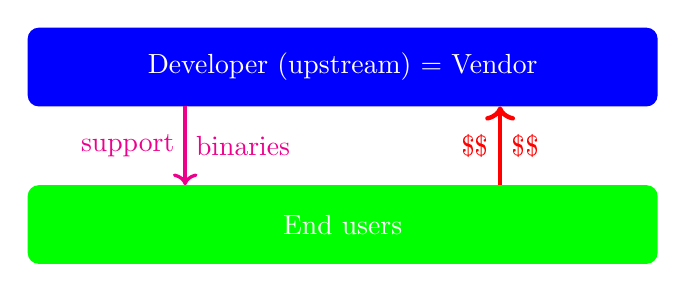
\begin{tikzpicture}[scale=1, transform shape]
    \fill[fill=blue, text=white, rounded corners] (0, 0) rectangle ++(8, 1) node[pos=0.5] (A){Developer (upstream) = Vendor};
    \fill[fill=green, text=white, rounded corners] (0, -2) rectangle ++(8, 1) node[pos=0.5] (B){End users};
    \draw [red, ultra thick, ->] (6, -1) -- ++(0, 1) node [midway, left] {\$\$} node [midway, right] {\$\$};
    \draw [magenta, very thick, ->] (2, 0) -- node [midway, right, text centered] {binaries} node [midway, left, text centered] {support} ++(0, -1) ;
  \end{tikzpicture}
  \end{center}
  \end{figure}
\end{frame}
\begin{frame}[c]{The developer---user relationship: free software}
  \begin{figure}[h]
  \begin{center}
  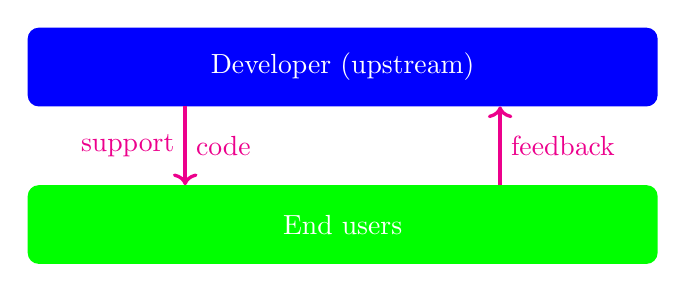
\begin{tikzpicture}[scale=1, transform shape]
    \fill[fill=blue, text=white, rounded corners] (0, 0) rectangle ++(8, 1) node[pos=0.5] (A){Developer (upstream)};
    \fill[fill=green, text=white, rounded corners] (0, -2) rectangle ++(8, 1) node[pos=0.5] (B){End users};
    \draw [magenta, very thick, ->] (2, 0) -- node [midway, right, text centered] {code} node [midway, left, text centered] {support} ++(0, -1) ;
    \draw [magenta, very thick, ->] (6, -1) -- node [midway, right, text centered] {feedback} ++(0, 1);
  \end{tikzpicture}
  \end{center}
  \end{figure}
\end{frame}
\begin{frame}[c]{The developer---user relationship: distributions}
  \begin{figure}[h]
  \begin{center}
  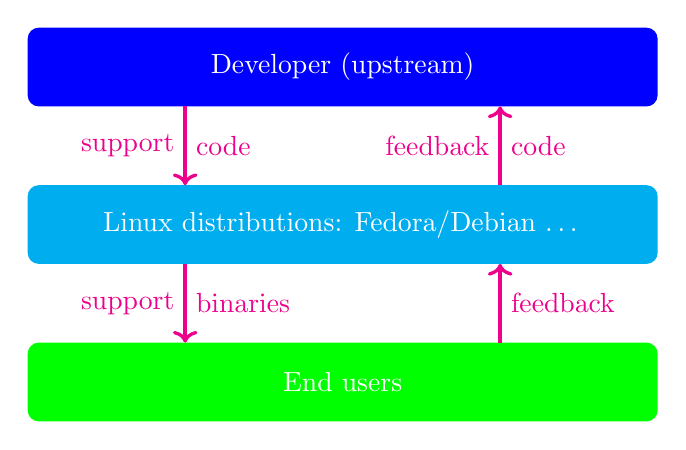
\begin{tikzpicture}[scale=1, transform shape]
    \fill[fill=blue, text=white, rounded corners] (0, 0) rectangle ++(8, 1) node[pos=0.5] (A){Developer (upstream)};
    \fill[fill=cyan, text=white, rounded corners] (0, -2) rectangle ++(8, 1) node[pos=0.5] (B){Linux distributions: Fedora/Debian \ldots};
    \draw [magenta, very thick, ->] (2, 0) -- node [midway, right, text centered] {code} node [midway, left, text centered] {support} ++(0, -1) ;
    \draw [magenta, very thick, ->] (6, -1) -- node [midway, right, text centered] {code} node [midway, left, text centered] {feedback} ++(0, 1) ;
    \fill[fill=green, text=white, rounded corners] (0, -4) rectangle ++(8, 1) node[pos=0.5] (B){End users};
    \draw [magenta, very thick, ->] (2, -2) -- node [midway, right, text centered] {binaries} node [midway, left, text centered] {support} ++(0, -1) ;
    \draw [magenta, very thick, ->] (6, -3) -- node [midway, right, text centered] {feedback} ++(0, 1) ;
  \end{tikzpicture}
  \end{center}
  \end{figure}
\end{frame}
\begin{frame}[c]{Distributions: package maintainers}
  \begin{itemize}
    \item Build software:
      \begin{itemize}
        \item including all \alert{dependencies}.
      \end{itemize}
      \pause{}
    \item Check for \alert{correctness} (!).
      \pause{}
    \item \alert{Keep up} with upstream: updates, security fixes \ldots.
      \pause{}
    \item \alert{Connect} upstream to users.
      \pause{}
    \item \alert{Enable} upstream to improve their software\footnotemark{}.
  \end{itemize}
  \footnotetext[3]{\href{https://fedoraproject.org/wiki/Staying_close_to_upstream_projects}{Fedora project: staying close to upstream.}}
\end{frame}
\section{NeuroFedora}
\begin{frame}[c]{Goals}
  \begin{itemize}
    \item Enable \alert{free science}:
      \pause{}
      \begin{itemize}
        \item researchers (end-users):
          \begin{itemize}
            \item ready to use \alert{tested} tools.
          \end{itemize}
          \pause{}
        \item upstreams:
          \begin{itemize}
            \item feedback from users.
            \item software improvements.
            \item implement standards.
          \end{itemize}
      \end{itemize}
      \pause{}
    \item Help make science \alert{\enquote{default to open}}.
  \end{itemize}
\end{frame}
\begin{frame}[c]{NeuroFedora example I\@: NEST (\(\bigstar\bigstar\bigstar\bigstar\bigstar\))}
  \begin{itemize}
    \item Build requires\footnotemark:
      \begin{itemize}
        \item \alert{Compulsory:} Python+, Cython, GSL, Ncurses, CMake, GCC\@.
          \pause{}
        \item \alert{Optional:} libneurosim (for PyNN), MUSIC, MPICH, OpenMPI\@.
      \end{itemize}
  \end{itemize}
  \footnotetext[4]{\href{https://src.fedoraproject.org/rpms/nest/blob/master/f/nest.spec}{Fedora project: nest SPEC file.}}
\end{frame}
\begin{frame}[c]{NeuroFedora Example I\@: NEST\@: usage}
  \texttt{\$ sudo dnf install python3-nest}\\
  \texttt{\$ sudo dnf install python3-nest-mpich}\\
  \texttt{\$ sudo dnf install python3-nest-openmpi}
\end{frame}
\begin{frame}[c]{NeuroFedora example II\@: PyNN (\(\bigstar\bigstar\bigstar\))}
  \begin{itemize}
    \item Build requires\footnotemark:
      \pause{}
      \begin{itemize}
        \item \alert{Compulsory:} Python+, Ncurses, CMake, GCC\@.
        \item \alert{At least one of:} NEST, Brian, NEURON\@.
      \end{itemize}
  \end{itemize}
  \footnotetext[5]{\href{https://github.com/sanjayankur31/rpm-specs/blob/python-pynn/python-PyNN.spec}{Fedora project: PyNN SPEC file (WIP).}}
\end{frame}
\begin{frame}[c]{NeuroFedora Example II\@: PyNN (WIP): usage}
  \texttt{\$ sudo dnf install python3-PyNN}

  Installs PyNN and NEST, Brian\footnotemark{}, NineML (and NEURON\footnotemark{}).

  \pause{}
  \texttt{\$ sudo dnf install python3-PyNN-nest}

  Installs PyNN and NEST\@.
  \footnotetext[6]{Requires Brian v1}
  \footnotetext[7]{\href{https://github.com/neuronsimulator/nrn/issues/113}{WIP: Requires upstream improvements.}}
\end{frame}
\begin{frame}[c]{NeuroFedora: package metrics}
  \begin{itemize}
    \item 67 packages available in total\footnotemark.
    \item \textasciitilde{}130 in queue\footnotemark.
  \end{itemize}
  \footnotetext[8]{\href{https://src.fedoraproject.org/group/neuro-sig}{src.fedoraproject.org: Neuro-SIG}}
  \footnotetext[9]{\href{https://pagure.io/neuro-sig/NeuroFedora/issues?status=Open}{Pagure.io: Neuro-SIG: issues}}
\end{frame}
\begin{frame}[c]{NeuroFedora: computational neuroscience}
  \begin{itemize}
    \item Available: NEST, NineML, moose, Brian2, PyLEMS\@.
    \item In queue (26)\footnotemark: NEURON, PyNN, Brian1, NetPyne, Genesis, NeuroMLlite, pyNeuroML, pype9, HNN, libSBML \ldots
  \end{itemize}
  \footnotetext[10]{\href{https://pagure.io/neuro-sig/NeuroFedora/issues?tags=F\%3A+Computational+neuroscience}{Neuro-SIG: computational neuroscience}}
\end{frame}
\begin{frame}[c]{NeuroFedora: neuroimaging}
  \begin{itemize}
    \item Available: biosig, dcm2niix, gifticlib, InsightToolKit, libminc, dipy, fsleyes, mne-bids, pydicom \ldots
    \item In queue (40)\footnotemark: Nistats, FEAT, TranctoR, FSL, SPM, connectomeviewer, nipype, itktools \ldots
  \end{itemize}
  \footnotetext[11]{\href{https://pagure.io/neuro-sig/NeuroFedora/issues?status=Open&tags=F\%3A+Neuroimaging&priority=0}{Neuro-SIG: neuroimaging}}
\end{frame}
\begin{frame}[c]{NeuroFedora: data analysis}
  \begin{itemize}
    \item Available: nilearn, scikit-learn, klusta, lazyarray, neo, nitime, patsy \ldots
    \item In queue (25)\footnotemark: spyke-viewer, stimfit, pyelectro, pyspike, pymc3 \ldots
  \end{itemize}
  \footnotetext[12]{\href{https://pagure.io/neuro-sig/NeuroFedora/issues?tags=F\%3A+Data+Analysis}{Neuro-SIG: data analysis}}
\end{frame}
\begin{frame}[c]{NeuroFedora: utilities}
  \begin{itemize}
    \item Available: texlive (full), duecredit, chaospy, \ldots
    \item In queue (37)\footnotemark: spiking-circus, pingouin, spykeutils, PsychToolbox, tridesclous, uncertainpy, neuroshare, Btmorph \ldots
  \end{itemize}
  \footnotetext[13]{\href{https://pagure.io/neuro-sig/NeuroFedora/issues?tags=F\%3A+Utilities}{Neuro-SIG: utilities}}
\end{frame}
\begin{frame}[c]{NeuroFedora: plans}
  \begin{itemize}
    \item Continue package imports.
      \pause{}
    \item Update documentation\footnotemark.
      \pause{}
    \item Docker images\footnotemark!
      \pause{}
    \item Announce to research community.
      \pause{}
    \item RHEL/CentOS/Scientific Linux support (our cluster runs Scientific Linux).
      \pause{}
    \item BoFs/Hack sessions at scientific conferences (workshop at CNS 2019?)
  \end{itemize}
  \footnotetext[14]{\href{https://pagure.io/neuro-sig/documentation}{Pagure.io: Neuro-SIG: Documentation}}
  \footnotetext[15]{\href{https://registry.fedoraproject.org/}{registry.fedoraproject.org}}
\end{frame}
\begin{frame}[c]{NeuroFedora: requirements}
  \begin{itemize}
    \item More package maintainers\footnotemark.
      \pause{}
    \item Testers---end users who are happy to test packages and provide feedback (QA)\footnotemark.
      \pause{}
    \item Documentation writers/proofreaders.
  \end{itemize}
  \footnotetext[16]{\href{https://fedoraproject.org/wiki/Join_the_package_collection_maintainers}{Fedora: Join the package maintainers}}
  \footnotetext[17]{\href{https://fedoraproject.org/wiki/QA:Updates_Testing}{Fedora QA: testing updates}}
\end{frame}
\begin{frame}[c]{NeuroFedora}
  \begin{center}
    https://fedoraproject.org/wiki/SIGs/NeuroFedora\vspace{0.2cm}

    \href{http://creativecommons.org/licenses/by-sa/4.0/}{Creative Commons Attribution-ShareAlike 4.0 International License}.\vspace{0.2cm}

    \ccbysa{}
  \end{center}
\end{frame}
\end{document}

